\documentclass[12pt]{article}

\usepackage{fullpage}
\usepackage{amsmath}
\usepackage{amssymb}
\usepackage{libertine}
\usepackage{polynom}
\usepackage{tikz}

\title{Stewart Calculus Review}
\author{Brandon Munshaw}

\begin{document}

\maketitle

\section{Review}

\subsection{Quadratic Formula}

\begin{align*}
ax^2+bx+c=0\\
\implies x=\frac{-b\pm\sqrt{b^2-4ac}}{2a}
\end{align*}
\emph{Proof}

\begin{align*}
  &ax^2+bx+c=0\\
  \implies &x^2+\frac{b}{a}x = - \frac{c}{a}\\
  \implies &(x)^2+2(x)\bigg(\frac{b}{2a}\bigg) = -\frac{c}{a}\\
  \implies &(x)^2+2(x)\bigg(\frac{b}{2a}\bigg)+\bigg(\frac{b}{2a}\bigg)^2 = \bigg(\frac{b}{2a}\bigg)^2-\frac{c}{a}\\
  &\text{Recall } (\alpha+\beta)^2=\alpha^2+2\alpha\beta+\beta^2\\
  \implies &\bigg(x+\frac{b}{2a}\bigg)^2 = \frac{b^2-4ac}{(2a)^2}\\
  \implies &x = \frac{-b\pm\sqrt{b^2-4ac}}{2a}
\end{align*}

\subsection{Polynomial Factorization}

Factor $P(x)=12x^3-32x^2+25x-6$.

\emph{Solution}

\begin{align*}
  &\text{Rational solution } x \in \bigg\{\pm\frac{p}{q}:p|12,q|6\bigg\}\\
  \implies &x\in\pm\frac{1,2,3,4}{1,2,3}\\
  &\text{By trial and error } P(2/3) = 0 \implies 2x-3 \text{ is a factor.}\\
  &\text{\polylongdiv{12x^3-32x^2+25x-6}{2x-3}}\\
  &(2x-3)(6x^2-7x+2)\\
  =&(2x-3)[(6x^2-4x)-(3x-2)]\\
  =&(2x-3)[2x(3x-2)-(3x-2)]\\
  =&(2x-3)(2x-1)(3x-2)
\end{align*}

\subsection{Partial Fraction Decomposition}

Decompose $$\frac{x-2}{(x^2+x+1)(x+1)}$$ into partial fractions.

\emph{Solution}

\begin{align*}
  &\frac{x-2}{(x^2+x+1)(x+1)} = \frac{Ax+B}{x^2+x+1} + \frac{C}{x+1}\\
  \implies&x-2 = (Ax+B)(x+1) + C(x^2+x+1)\\
  \implies&x-2 = (A+C)x^2+(A+B+C)x+(B+C)\\
  \implies&A+C=0\\
  &A+B+C=1\\
  &B+C=-2\\
  \implies&A=3,~B=1,~C=-3\\
  \therefore~&\frac{x-2}{(x^2+x+1)(x+1)} = \frac{3x+1}{x^2+x+1} - \frac{3}{x+1}
\end{align*}

\subsection{Pythagorean Theorem}

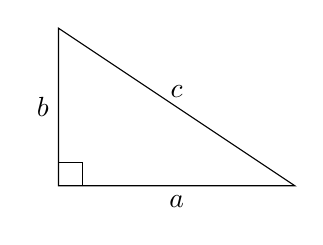
\begin{tikzpicture}
  \draw (0,0)
    -- (3,0) node[midway,below] {$a$}
    -- (0,2) node[midway,above] {$c$}
    -- cycle node[midway,left] {$b$};
  \draw (0.3,0)
    -- (0.3,0.3)
    -- (0,0.3);
\end{tikzpicture}

$\implies a^2+b^2=c^2$

\emph{Proof}

Construct the following figures. They have the same area $(a+b)^2$. Subtract 4 triangles from both figures, and see the $c$-square has the same area as the $a$-square and the $b$-square.

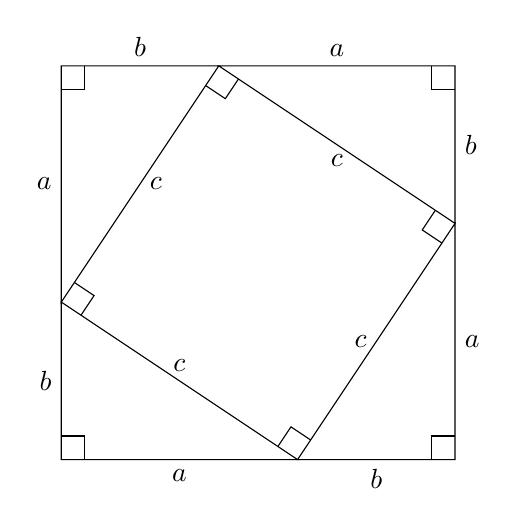
\begin{tikzpicture}
  \draw (0,0)
  -- (3,0) node[midway,below] {$a$}
  -- (0,2) node[midway,above] {$c$}
  -- cycle node[midway,left] {$b$};
  \draw (0.3,0)
  -- (0.3,0.3)
  -- (0,0.3);
  \draw (0.2496,1.8336)
  -- (0.416,2.0832)
  -- (0.1664,2.2496);

  \draw (0,2)
  -- (0,5) node[midway,left] {$a$}
  -- (2,5) node[midway,above] {$b$}
  -- cycle node[midway,right] {$c$};
  \draw (0,4.7)
  -- (0.3,4.7)
  -- (0.3,5);
  \draw (1.8336,4.7504)
  -- (2.0832,4.584)
  -- (2.2496,4.8336);

  \draw (2,5)
  -- (5,5) node[midway,above] {$a$}
  -- (5,3) node[midway,right] {$b$}
  -- cycle node[midway,below] {$c$};
  \draw (4.7,5)
  -- (4.7,4.7)
  -- (5,4.7);
  \draw (4.7504,3.1664)
  -- (4.584,2.9168)
  -- (4.8336,2.7504);

  \draw (5,3)
  -- (5,0) node[midway,right] {$a$}
  -- (3,0) node[midway,below] {$b$}
  -- cycle node[midway,left] {$c$};
  \draw (5,0.3)
  -- (4.7,0.3)
  -- (4.7,0);
  \draw (2.7504,0.1664)
  -- (2.9168,0.416)
  -- (3.1664,0.2496);
\end{tikzpicture}
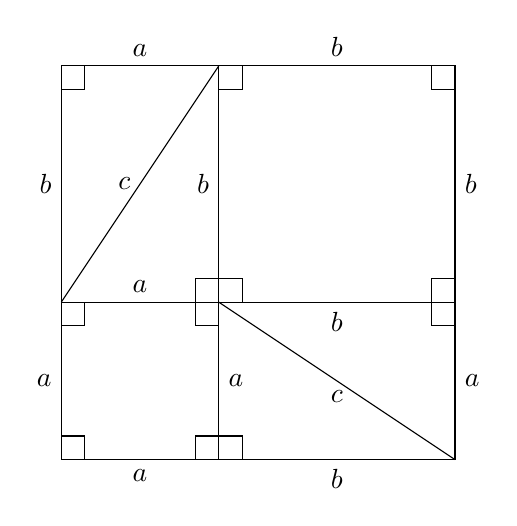
\begin{tikzpicture}
  \draw (0,0)
  -- (0,2) node[midway,left] {$a$}
  -- (0,5) node[midway,left] {$b$}
  -- (2,5) node[midway,above] {$a$}
  -- (5,5) node[midway,above] {$b$}
  -- (5,2) node[midway,right] {$b$}
  -- (5,0) node[midway,right] {$a$}
  -- (2,0) node[midway,below] {$b$}
  -- cycle node[midway,below] {$a$};

  \draw (0,0.3)
  -- (0.3,0.3)
  -- (0.3,0);
  \draw (0,4.7)
  -- (0.3,4.7)
  -- (0.3,5);
  \draw (4.7,5)
  -- (4.7,4.7)
  -- (5,4.7);
  \draw (2,1.7)
  -- (1.7,1.7)
  -- (1.7,2.3)
  -- (2.3,2.3)
  -- (2.3,2);
  \draw (1.7,0)
  -- (1.7,0.3)
  -- (2.3,0.3)
  -- (2.3,0);
  \draw (5,1.7)
  -- (4.7,1.7)
  -- (4.7,2.3)
  -- (5,2.3);
  \draw (0,1.7)
  -- (0.3,1.7)
  -- (0.3,2);
  \draw (2,4.7)
  -- (2.3,4.7)
  -- (2.3,5);

  \draw (2,0)
  -- (2,2) node[midway,right] {$a$}
  -- (2,5) node[midway,left] {$b$};
  \draw (0,2)
  -- (2,2) node[midway,above] {$a$}
  -- (5,2) node[midway,below] {$b$};
  \draw (2,2)
  -- (5,0) node[midway,below] {$c$};
  \draw (0,2)
  -- (2,5) node[midway,left] {$c$};
\end{tikzpicture}

\subsection{Trigonometry}

\begin{align*}
  \sin \theta  &= \frac{\text{opp}}{\text{hyp}} & \csc \theta  &= \frac{\text{hyp}}{\text{opp}}\\
  \cos \theta  &= \frac{\text{adj}}{\text{hyp}} & \sec \theta  &= \frac{\text{hyp}}{\text{adj}}\\
  \tan \theta  &= \frac{\text{opp}}{\text{adj}} & \cot \theta  &= \frac{\text{adj}}{\text{opp}}\\
\end{align*}

\subsubsection{Pythagorean Identities}

\begin{align*}
  \sin^2 \theta + \cos^2 \theta = 1\\
  1+\tan^2 \theta = \sec^2 \theta\\
  1+cot^2 \theta = \csc^2 \theta
\end{align*}

\emph{Proof}

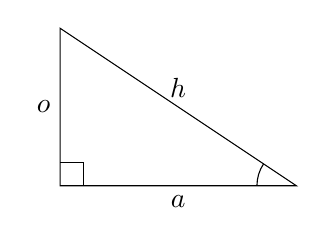
\begin{tikzpicture}
  \draw (0,0)
  -- (3,0) node[midway,below] {$a$}
  -- (0,2) node[midway,above] {$h$}
  -- cycle node[midway,left] {$o$};
  \draw (0.3,0)
  -- (0.3,0.3)
  -- (0,0.3);
  \draw (2.5,0)
  arc [start angle = 180, end angle = 146.31, x radius = 0.5, y radius = 0.5];
\end{tikzpicture}
\begin{align*}
  \implies & h^2=o^2+a^2\\
  \implies & 1 = \bigg(\frac{o}{h}\bigg)^2 + \bigg(\frac{o}{h}\bigg)^2\\
  \implies & \sin^2 \theta + \cos^2 \theta = 1
\end{align*}

\subsubsection{Law of Sines}

\begin{tikzpicture}
  \draw (0,0) node[left] {$A$}
  -- (1,2) node[above] {$B$} node[midway,left] {$c$}
  -- (4,0) node[right] {$C$} node[midway,above] {$a$}
  -- cycle node[midway,below] {$b$};
\end{tikzpicture}

\[
  \implies \frac{\sin A}{a} = \frac{\sin B}{b} = \frac{\sin C}{c}
\]

\emph{Proof}

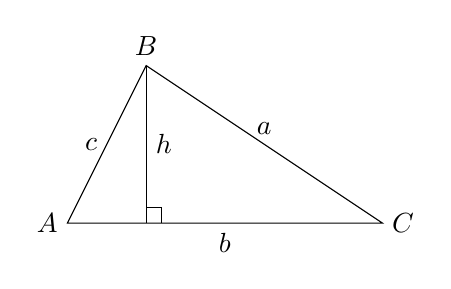
\begin{tikzpicture}
  \draw (0,0) node[left] {$A$}
  -- (1,2) node[above] {$B$} node[midway,left] {$c$}
  -- (4,0) node[right] {$C$} node[midway,above] {$a$}
  -- cycle node[midway,below] {$b$};
  \draw (1,2)
  -- (1,0) node[midway,right] {$h$};
  \draw (1,0.2)
  -- (1.2,0.2)
  -- (1.2,0);
\end{tikzpicture}

\begin{align*}
  \implies & h = c \sin A\\
  & h = a \sin C\\
  \implies &\frac{\sin A}{a} = \frac{\sin C}{c}
\end{align*}

\subsubsection{Law of Cosines}

\begin{tikzpicture}
  \draw (0,0) node[left] {$A$}
  -- (1,2) node[above] {$B$} node[midway,left] {$c$}
  -- (4,0) node[right] {$C$} node[midway,above] {$a$}
  -- cycle node[midway,below] {$b$};
\end{tikzpicture}

\[
  \implies c^2=a^2+b^2-2ab\cos C
\]

\emph{Proof}

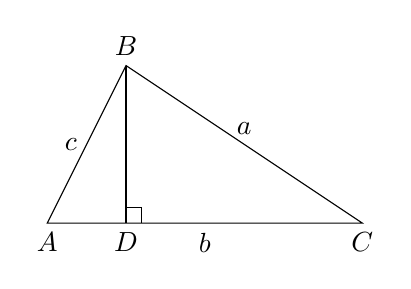
\begin{tikzpicture}
  \draw (0,0) node[below] {$A$}
  -- (1,2) node[above] {$B$} node[midway,left] {$c$}
  -- (4,0) node[below] {$C$} node[midway,above] {$a$}
  -- cycle node[midway,below] {$b$};
  \draw (1,2)
  -- (1,0) node[below] {$D$};
  \draw (1,0.2)
  -- (1.2,0.2)
  -- (1.2,0);
\end{tikzpicture}

\begin{align*}
  \implies & \overline{BD} = a \sin C\\
  & \overline{AD} = b - a \cos C\\
  \text{Since } & c^2=\overline{AD}^2+\overline{BD+}^2\\
  \implies & c^2 = (b-a\cos C)^2+(a \sin C)^2\\
  \implies & c^2 = b^2 -2ab \cos C + a^2 \cos^2 C + a^2 \sin^2 C\\
  \implies & c^2=b^2-2ab \cos C + a^2(\cos^2 C + \sin^2 C)\\
  \implies & c^2=a^2+b^2-2ab \cos C
\end{align*}

\subsubsection{Angle Addition Identities}

\begin{align*}
  \sin(x \pm y) &= \sin x \cos y \pm \cos x \sin y\\
  \cos(x \pm y) &= \cos x \cos y \mp \sin x \sin y\\
  \tan(x \pm y) &= \frac{\tan x \pm \tan y}{1 \mp \tan x \tan y}
\end{align*}

\emph{Proof}

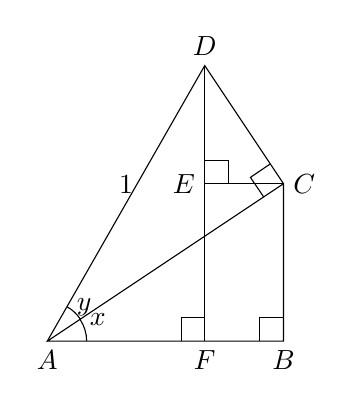
\begin{tikzpicture}
  \draw (0,0) node[below] {$A$}
  -- (3,0) node[below] {$B$}
  -- (3,2) node[right] {$C$}
  -- cycle;

  \draw (0.5,0)
  arc [start angle = 0, end angle = 33.69, x radius = 0.5, y radius = 0.5]
  node [right] {$x$};

  \draw (2.7,0)
  -- (2.7,0.3)
  -- (3,0.3);

  \draw (3,2)
  -- (2,3.5) node[above] {$D$}
  -- (0,0) node[midway,above] {1};

  \draw (2.75,1.83)
  -- (2.58,2.08)
  -- (2.83,2.25);

  \draw (0.42,.28)
  arc [start angle = 33.69, end angle = 60.26, x radius = 0.5, y radius = 0.5]
  node [right] {$y$};

  \draw (2,3.5)
  -- (2,2) node [left] {$E$}
  -- (2,0) node [below] {$F$};

  \draw (2,2)
  -- (3,2);

  \draw (2,2.3)
  -- (2.3,2.3)
  -- (2.3,2);

  \draw (2,0.3)
  -- (1.7,0.3)
  -- (1.7,0);
\end{tikzpicture}

\begin{align*}
  \implies &\sin(x+y) = \overline{DF} = \overline{DE} + \overline{EF} = \overline{DE} + \overline{CB}\\
           & \overline{DC} = \sin y\\
           & \overline{AC} = \cos y\\
           & \overline{CB} = \sin x \cos y\\
           & \angle ECA = x\\
           & \angle DCE = \frac{\pi}{2}-x\\
           & \angle EDC = x\\
           & \overline{DE} = \cos x \sin y\\
  \implies & \sin(x+y) = \sin x \cos y + \cos x \sin y\\
\end{align*}

\subsubsection{Double-Angle and Half-Angle Formulas}

\begin{align*}
  \sin 2x &= 2 \sin x \cos x\\
  \cos 2x &= \cos^2 x - \sin^2 x\\
          &= 2 \cos^2 x - 1\\
          &= 1 - 2 \sin^2 x\\
  \tan 2x &= \frac{2 \tan x}{1 - \tan^2 x}\\
  \sin^2 x &= \frac{1-\cos 2x}{2}\\
  \cos^2 x &= \frac{1+\cos^2 2x}{2}
\end{align*}

\section{Limits}

\subsection{Definition of Limit}

\[
  \lim_{x \to a} f(x) = L \iff \forall \epsilon > 0, \exists \delta > 0 \ni (0 < |x - a| < \delta => |f(x)-L| < \epsilon)
\]

\end{document}